

\color{black}
\subsection*{Inference with Markov models}

Recall the state transition diagram and transition probability matrix of a Markov chain ${\lambda_1}$ which models the behavior of an NPC who is ``patrolling the map''
\begin{center}
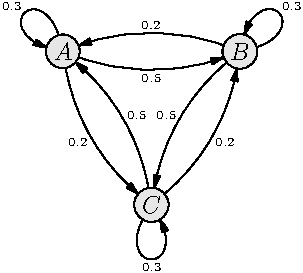
\includegraphics[width=0.4\textwidth]{dungeonMC1.pdf}
\qquad
\raisebox{2.5cm}{$\mat{P}_{\lambda_1} = \begin{bmatrix} 0.3 & 0.2 & 0.5 \\ 0.5 & 0.3 & 0.2 \\ 0.2 & 0.5 & 0.3 \end{bmatrix}$}
\end{center}

The probability of the event $E_1 = $ ``the NPC goes from room $C$ to room $B$ and then to room $A$'' amounts to
\begin{align*}
\prob{E_1} & = \cprob{X_1 = B}{X_0 = C} \cdot \cprob{X_2 = A}{X_1 = B}
\intertext{and the corresponding log-likelihood amounts to}
\mathcal{L} \bigl( E_1 \bigr) & =  \ln \cprob{X_1 = B}{X_0 = C} + \ln \cprob{X_2 = A}{X_1 = B}
\end{align*}

Compute both these values for the model $\lambda_1$. Round your results to \emph{two} decimal places.
\color{blue}
%%%%%
%%%%% enter your results after the '=' signs
%%%%%
\begin{equation*}
\prob{E_1} = 0.04
\end{equation*}
\begin{equation*}
\mathcal{L} \bigl( E_1 \bigr) = -3.22
\end{equation*}
%%%%%
%%%%%
%%%%%
\color{black}




Also for model $\lambda_1$, compute the probability and log-likelihood of the event $E_2 = $ ``the NPC goes from room $C$ to room $A$ and then to room $B$''
\color{blue}
%%%%%
%%%%% enter your results after the '=' signs
%%%%%
\begin{equation*}
\prob{E_2} = 0.25
\end{equation*}
\begin{equation*}
\mathcal{L} \bigl( E_2 \bigr) = -1.39
\end{equation*}
%%%%%
%%%%%
%%%%%
\color{black}
\newpage




